\documentclass[]{article}
\usepackage{lmodern}
\usepackage{amssymb,amsmath}
\usepackage{ifxetex,ifluatex}
\usepackage{fixltx2e} % provides \textsubscript
\ifnum 0\ifxetex 1\fi\ifluatex 1\fi=0 % if pdftex
  \usepackage[T1]{fontenc}
  \usepackage[utf8]{inputenc}
\else % if luatex or xelatex
  \ifxetex
    \usepackage{mathspec}
  \else
    \usepackage{fontspec}
  \fi
  \defaultfontfeatures{Ligatures=TeX,Scale=MatchLowercase}
\fi
% use upquote if available, for straight quotes in verbatim environments
\IfFileExists{upquote.sty}{\usepackage{upquote}}{}
% use microtype if available
\IfFileExists{microtype.sty}{%
\usepackage{microtype}
\UseMicrotypeSet[protrusion]{basicmath} % disable protrusion for tt fonts
}{}
\usepackage[margin=1in]{geometry}
\usepackage{hyperref}
\hypersetup{unicode=true,
            pdftitle={Homework 9},
            pdfauthor={Christophe Hunt},
            pdfborder={0 0 0},
            breaklinks=true}
\urlstyle{same}  % don't use monospace font for urls
\usepackage{color}
\usepackage{fancyvrb}
\newcommand{\VerbBar}{|}
\newcommand{\VERB}{\Verb[commandchars=\\\{\}]}
\DefineVerbatimEnvironment{Highlighting}{Verbatim}{commandchars=\\\{\}}
% Add ',fontsize=\small' for more characters per line
\usepackage{framed}
\definecolor{shadecolor}{RGB}{248,248,248}
\newenvironment{Shaded}{\begin{snugshade}}{\end{snugshade}}
\newcommand{\KeywordTok}[1]{\textcolor[rgb]{0.13,0.29,0.53}{\textbf{{#1}}}}
\newcommand{\DataTypeTok}[1]{\textcolor[rgb]{0.13,0.29,0.53}{{#1}}}
\newcommand{\DecValTok}[1]{\textcolor[rgb]{0.00,0.00,0.81}{{#1}}}
\newcommand{\BaseNTok}[1]{\textcolor[rgb]{0.00,0.00,0.81}{{#1}}}
\newcommand{\FloatTok}[1]{\textcolor[rgb]{0.00,0.00,0.81}{{#1}}}
\newcommand{\ConstantTok}[1]{\textcolor[rgb]{0.00,0.00,0.00}{{#1}}}
\newcommand{\CharTok}[1]{\textcolor[rgb]{0.31,0.60,0.02}{{#1}}}
\newcommand{\SpecialCharTok}[1]{\textcolor[rgb]{0.00,0.00,0.00}{{#1}}}
\newcommand{\StringTok}[1]{\textcolor[rgb]{0.31,0.60,0.02}{{#1}}}
\newcommand{\VerbatimStringTok}[1]{\textcolor[rgb]{0.31,0.60,0.02}{{#1}}}
\newcommand{\SpecialStringTok}[1]{\textcolor[rgb]{0.31,0.60,0.02}{{#1}}}
\newcommand{\ImportTok}[1]{{#1}}
\newcommand{\CommentTok}[1]{\textcolor[rgb]{0.56,0.35,0.01}{\textit{{#1}}}}
\newcommand{\DocumentationTok}[1]{\textcolor[rgb]{0.56,0.35,0.01}{\textbf{\textit{{#1}}}}}
\newcommand{\AnnotationTok}[1]{\textcolor[rgb]{0.56,0.35,0.01}{\textbf{\textit{{#1}}}}}
\newcommand{\CommentVarTok}[1]{\textcolor[rgb]{0.56,0.35,0.01}{\textbf{\textit{{#1}}}}}
\newcommand{\OtherTok}[1]{\textcolor[rgb]{0.56,0.35,0.01}{{#1}}}
\newcommand{\FunctionTok}[1]{\textcolor[rgb]{0.00,0.00,0.00}{{#1}}}
\newcommand{\VariableTok}[1]{\textcolor[rgb]{0.00,0.00,0.00}{{#1}}}
\newcommand{\ControlFlowTok}[1]{\textcolor[rgb]{0.13,0.29,0.53}{\textbf{{#1}}}}
\newcommand{\OperatorTok}[1]{\textcolor[rgb]{0.81,0.36,0.00}{\textbf{{#1}}}}
\newcommand{\BuiltInTok}[1]{{#1}}
\newcommand{\ExtensionTok}[1]{{#1}}
\newcommand{\PreprocessorTok}[1]{\textcolor[rgb]{0.56,0.35,0.01}{\textit{{#1}}}}
\newcommand{\AttributeTok}[1]{\textcolor[rgb]{0.77,0.63,0.00}{{#1}}}
\newcommand{\RegionMarkerTok}[1]{{#1}}
\newcommand{\InformationTok}[1]{\textcolor[rgb]{0.56,0.35,0.01}{\textbf{\textit{{#1}}}}}
\newcommand{\WarningTok}[1]{\textcolor[rgb]{0.56,0.35,0.01}{\textbf{\textit{{#1}}}}}
\newcommand{\AlertTok}[1]{\textcolor[rgb]{0.94,0.16,0.16}{{#1}}}
\newcommand{\ErrorTok}[1]{\textcolor[rgb]{0.64,0.00,0.00}{\textbf{{#1}}}}
\newcommand{\NormalTok}[1]{{#1}}
\usepackage{graphicx,grffile}
\makeatletter
\def\maxwidth{\ifdim\Gin@nat@width>\linewidth\linewidth\else\Gin@nat@width\fi}
\def\maxheight{\ifdim\Gin@nat@height>\textheight\textheight\else\Gin@nat@height\fi}
\makeatother
% Scale images if necessary, so that they will not overflow the page
% margins by default, and it is still possible to overwrite the defaults
% using explicit options in \includegraphics[width, height, ...]{}
\setkeys{Gin}{width=\maxwidth,height=\maxheight,keepaspectratio}
\IfFileExists{parskip.sty}{%
\usepackage{parskip}
}{% else
\setlength{\parindent}{0pt}
\setlength{\parskip}{6pt plus 2pt minus 1pt}
}
\setlength{\emergencystretch}{3em}  % prevent overfull lines
\providecommand{\tightlist}{%
  \setlength{\itemsep}{0pt}\setlength{\parskip}{0pt}}
\setcounter{secnumdepth}{5}
% Redefines (sub)paragraphs to behave more like sections
\ifx\paragraph\undefined\else
\let\oldparagraph\paragraph
\renewcommand{\paragraph}[1]{\oldparagraph{#1}\mbox{}}
\fi
\ifx\subparagraph\undefined\else
\let\oldsubparagraph\subparagraph
\renewcommand{\subparagraph}[1]{\oldsubparagraph{#1}\mbox{}}
\fi

%%% Use protect on footnotes to avoid problems with footnotes in titles
\let\rmarkdownfootnote\footnote%
\def\footnote{\protect\rmarkdownfootnote}

%%% Change title format to be more compact
\usepackage{titling}

% Create subtitle command for use in maketitle
\newcommand{\subtitle}[1]{
  \posttitle{
    \begin{center}\large#1\end{center}
    }
}

\setlength{\droptitle}{-2em}
  \title{Homework 9}
  \pretitle{\vspace{\droptitle}\centering\huge}
  \posttitle{\par}
  \author{Christophe Hunt}
  \preauthor{\centering\large\emph}
  \postauthor{\par}
  \predate{\centering\large\emph}
  \postdate{\par}
  \date{April 1, 2017}

\usepackage{relsize}
\usepackage{setspace}
\usepackage{amsmath,amsfonts,amsthm}
\usepackage[sfdefault]{roboto}
\usepackage[T1]{fontenc}
\usepackage{float}
\usepackage{multirow}
\usepackage{mathtools}
\usepackage{tikz}

\begin{document}
\maketitle

{
\setcounter{tocdepth}{2}
\tableofcontents
}
This week, we'll empirically verify Central Limit Theorem. We'll write
code to run a small simulation on some distributions and verify that the
results match what we expect from Central Limit Theorem. Please use R
markdown to capture all your experiments and code. Please submit your
Rmd file with your name as the filename.

\newpage

\section{(1) produce a sample of random
variable}\label{produce-a-sample-of-random-variable}

First write a function that will produce a sample of random variable
that is distributed as follows:

\(f(x) = x, 0 \leq x \leq 1\)\\
\(f(x) = 2 - x, 1 < x \leq 2\)

That is, when your function is called, it will return a random variable
between 0 and 2 that is distributed according to the above PDF. Please
note that this is not the same as writing a function and sampling
uniformly from it. In the online session this week, I'll cover Sampling
techniques. You will find it useful when you do the assignment for this
week. In addition, as usual, there are one-liners in R that will give
you samples from a function. We'll cover both of these approaches in the
online session.

\begin{Shaded}
\begin{Highlighting}[]
\NormalTok{random <-}\StringTok{ }\NormalTok{function()\{}
          \NormalTok{num <-}\StringTok{ }\KeywordTok{runif}\NormalTok{(}\DecValTok{1}\NormalTok{, }\DataTypeTok{min =} \DecValTok{0}\NormalTok{, }\DataTypeTok{max =} \DecValTok{2}\NormalTok{) }
          \NormalTok{if(num >}\StringTok{ }\DecValTok{1} \NormalTok{&&}\StringTok{ }\NormalTok{num <=}\StringTok{ }\DecValTok{2}\NormalTok{)\{}
             \KeywordTok{return}\NormalTok{(}\DecValTok{2}\NormalTok{-num)}
            \NormalTok{\} else \{}
              \KeywordTok{return}\NormalTok{(num)}
            \NormalTok{\}}
          \NormalTok{\} }
\KeywordTok{random}\NormalTok{()}
\end{Highlighting}
\end{Shaded}

\begin{verbatim}
## [1] 0.6448829
\end{verbatim}

\section{(2) produce a sample of random
variable}\label{produce-a-sample-of-random-variable-1}

Now, write a function that will produce a sample of random variable that
is distributed as follows:

\(f(x) = 1 - x, 0 \leq x \leq 1\)\\
\(f(x) = x - 1, 1 < x \leq 2\)

\begin{Shaded}
\begin{Highlighting}[]
\NormalTok{random2 <-}\StringTok{ }\NormalTok{function()\{}
          \NormalTok{num <-}\StringTok{ }\KeywordTok{runif}\NormalTok{(}\DecValTok{1}\NormalTok{, }\DataTypeTok{min =} \DecValTok{0}\NormalTok{, }\DataTypeTok{max =} \DecValTok{2}\NormalTok{) }
          \NormalTok{if(num >}\StringTok{ }\DecValTok{1} \NormalTok{&&}\StringTok{ }\NormalTok{num <=}\StringTok{ }\DecValTok{2}\NormalTok{)\{}
             \KeywordTok{return}\NormalTok{(num}\DecValTok{-1}\NormalTok{)}
            \NormalTok{\} else \{}
              \KeywordTok{return}\NormalTok{(}\DecValTok{1}\NormalTok{-num)}
            \NormalTok{\}}
          \NormalTok{\} }
\KeywordTok{random2}\NormalTok{()}
\end{Highlighting}
\end{Shaded}

\begin{verbatim}
## [1] 0.2957906
\end{verbatim}

\section{(3) Draw 1000 samples}\label{draw-1000-samples}

Draw 1000 samples (call your function 1000 times each) from each of the
above two distributions and plot the resulting histograms. You should
have one histogram for each PDF. See that it matches your understanding
of these PDFs.

\begin{Shaded}
\begin{Highlighting}[]
\NormalTok{values <-}\StringTok{ }\KeywordTok{replicate}\NormalTok{(}\DecValTok{1000}\NormalTok{, }\KeywordTok{random}\NormalTok{())}
\KeywordTok{hist}\NormalTok{(values)}
\end{Highlighting}
\end{Shaded}

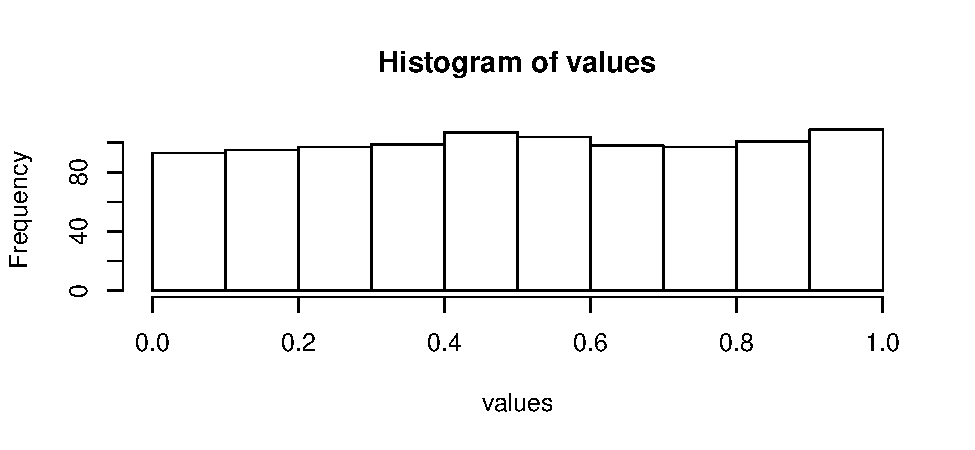
\includegraphics{CHunt_Assign9_PS1_PS2_files/figure-latex/unnamed-chunk-3-1.pdf}

\begin{Shaded}
\begin{Highlighting}[]
\NormalTok{values <-}\StringTok{ }\KeywordTok{replicate}\NormalTok{(}\DecValTok{1000}\NormalTok{, }\KeywordTok{random2}\NormalTok{())}
\KeywordTok{hist}\NormalTok{(values)}
\end{Highlighting}
\end{Shaded}

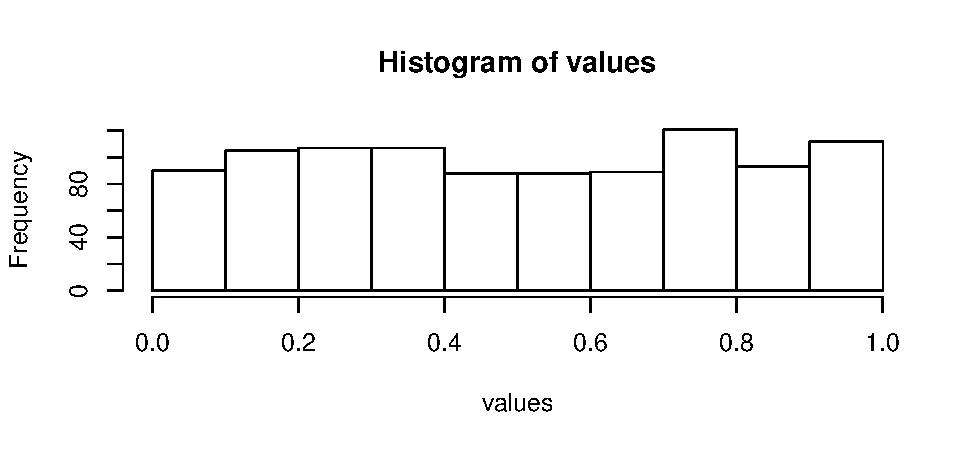
\includegraphics{CHunt_Assign9_PS1_PS2_files/figure-latex/unnamed-chunk-4-1.pdf}

\section{(4) Function to take means and generate
histogram}\label{function-to-take-means-and-generate-histogram}

Now, write a program that will take a sample set size n as a parameter
and the PDF as the second parameter, and perform 1000 iterations where
it samples from the PDF, each time taking n samples and computes the
mean of these n samples. It then plots a histogram of these 1000 means
that it computes.

\begin{Shaded}
\begin{Highlighting}[]
\NormalTok{means.hist <-}\StringTok{ }\NormalTok{function(n, PDF)\{}
          \NormalTok{x <-}\StringTok{ }\OtherTok{NULL}
          \NormalTok{for (i in }\DecValTok{1}\NormalTok{:}\DecValTok{1000}\NormalTok{)\{}
           \NormalTok{z <-}\StringTok{ }\KeywordTok{mean}\NormalTok{(}\KeywordTok{replicate}\NormalTok{(n, }\KeywordTok{PDF}\NormalTok{()))}
           \NormalTok{x <-}\StringTok{ }\KeywordTok{rbind}\NormalTok{(x, z)}
          \NormalTok{\}}
          \KeywordTok{hist}\NormalTok{(x)}
\NormalTok{\}}
\end{Highlighting}
\end{Shaded}

\subsection{Histogram of first random
function}\label{histogram-of-first-random-function}

\begin{Shaded}
\begin{Highlighting}[]
\KeywordTok{means.hist}\NormalTok{(}\DecValTok{30}\NormalTok{, }\DataTypeTok{PDF =} \NormalTok{random)}
\end{Highlighting}
\end{Shaded}

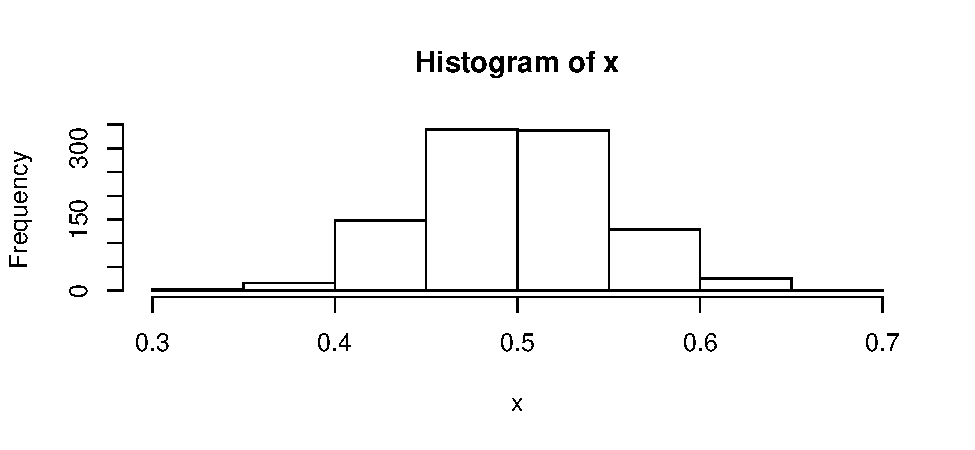
\includegraphics{CHunt_Assign9_PS1_PS2_files/figure-latex/unnamed-chunk-6-1.pdf}

\subsection{Histogram of second random
function}\label{histogram-of-second-random-function}

\begin{Shaded}
\begin{Highlighting}[]
\KeywordTok{means.hist}\NormalTok{(}\DecValTok{30}\NormalTok{, }\DataTypeTok{PDF =} \NormalTok{random2)}
\end{Highlighting}
\end{Shaded}

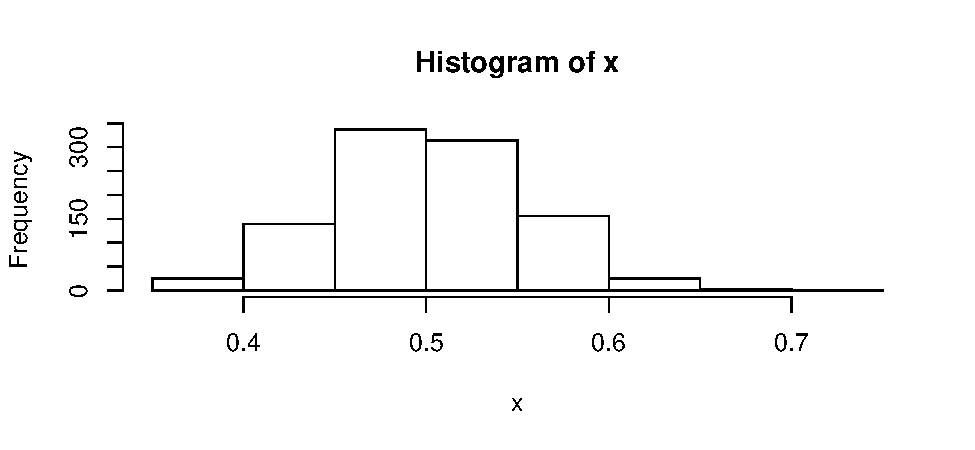
\includegraphics{CHunt_Assign9_PS1_PS2_files/figure-latex/unnamed-chunk-7-1.pdf}
\newpage

\section{(5) empirically verifying the Central Limit
Theorem}\label{empirically-verifying-the-central-limit-theorem}

Verify that as you set n to something like 10 or 20, each of the two
PDFs produce normally distributed mean of samples, empirically verifying
the Central Limit Theorem. Please play around with various values of n
and you'll see that even for reasonably small sample sizes such as 10,
Central Limit Theorem holds.

\begin{Shaded}
\begin{Highlighting}[]
\KeywordTok{means.hist}\NormalTok{(}\DecValTok{10}\NormalTok{, }\DataTypeTok{PDF =} \NormalTok{random)}
\end{Highlighting}
\end{Shaded}

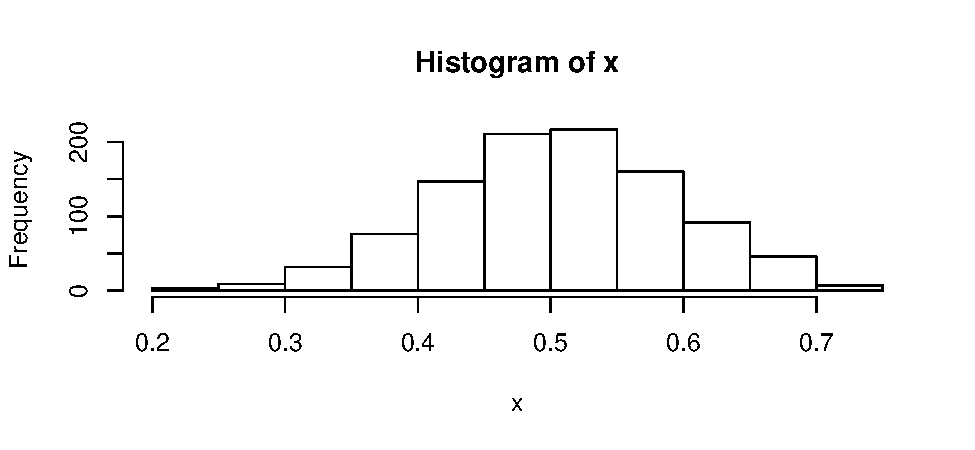
\includegraphics{CHunt_Assign9_PS1_PS2_files/figure-latex/unnamed-chunk-8-1.pdf}

\begin{Shaded}
\begin{Highlighting}[]
\KeywordTok{means.hist}\NormalTok{(}\DecValTok{10}\NormalTok{, }\DataTypeTok{PDF =} \NormalTok{random2)}
\end{Highlighting}
\end{Shaded}

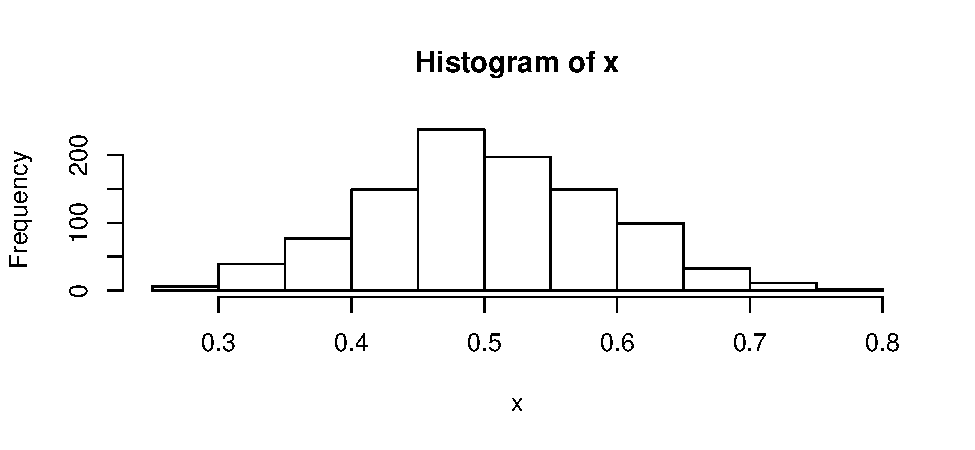
\includegraphics{CHunt_Assign9_PS1_PS2_files/figure-latex/unnamed-chunk-8-2.pdf}


\end{document}
